\documentclass[letterpaper, 11pt]{article}

\usepackage{lastpage, marginnote, siunitx, circuitikz, kantlipsum, hyperref, amsmath}
\def\UrlBreaks{\do\/\do-}

%\usepackage[hyphens]{url}

\usepackage{geometry}
\geometry{hscale=.6, vscale=.8, hmarginratio=2:1, vmarginratio=1:1, marginparwidth=.18\paperwidth, ignoremp}
%\geometry{marginparwidth=.1\paperwidth}

%\usepackage[T1]{fontenc}

\usepackage[explicit]{titlesec}
\titlespacing*{\section}{\dimexpr -\marginparsep-\marginparwidth}{*4}{*1}
\titleformat{\section}[runin]{\large\bfseries\titlerule[.5pt]\filright}{\makebox[1em][c]{\thesection}}{1em}{\parbox[t]{\dimexpr\marginparwidth-2em}{#1}\hskip\marginparsep\mbox{}}[\newline\vspace{-4ex}]

%\titlespacing*{\subsection}{\dimexpr -\marginparsep-\marginparwidth}{*4}{*1}
%\titleformat{\subsection}[runin]{\large\bfseries\titlerule[.5pt]\filright}{\makebox[1em][c]{\thesection}}{1em}{\parbox[t]{\dimexpr\marginparwidth-2em}{#1}\hskip\marginparsep\mbox{}}[\newline]

\usepackage{enumitem}
\newlist{steps}{enumerate}{1}
\setlist[steps]{label=Step \arabic*, font=\bfseries, leftmargin=-\marginparsep, itemindent=\marginparsep, align=right}

\usepackage{fancyhdr}
\pagestyle{fancy}
\fancyhf{}
\fancyhfoffset[lh,lf]{\dimexpr\marginparwidth+\marginparsep}
\fancyhf[lh]{UCD EEC 134}
\fancyhf[ch]{}
\fancyhf[rh]{}
%\fancyhf[lf]{left foot}
%\fancyhf[cf]{centre foot}
\fancyhf[rf]{Page \thepage /\pageref{LastPage}}
%\renewcommand{\footrulewidth}{.4pt}

%%%%%%%%%%%%%%%
%%%% Tikz definitions
%%%%%%%%%%%%%%%
%\tikzstyle{Uno}=[rectangle,fill=white,draw,line width=0.5mm]

%new commands
%display due date in red and link to the eec134-schedule.pdf document
\newcommand{\due}[1]{\href{https://github.com/ucdart/UCD-EEC134/blob/master/support/schedule/eec134-schedule.pdf}{\textcolor{red}{#1}}}

\graphicspath{{./figures/}}

\begin{document}

\title{Lab 2: Characterization of RF Amplifiers}
\author{Instructor: Xiaoguang ``Leo'' Liu\\lxgliu@ucdavis.edu \\
	\small \href{http://creativecommons.org/licenses/by-sa/4.0/}{CC BY-SA 4.0}}
\date{}
%\date{Last updated: \today}

\maketitle

The second lab revolves around the most common component in a RF/microwave system, the RF amplifier. RF amplifiers are used to amplify weak RF signal for either transmission or detection. They are designed differently depending on where they are used in the system. For example, low noise amplifiers (LNA) are usually used as the first stage of a receiver to minimize system noise; they are usually designed for the lowest noise possible, sometime even at the sacrifice of gain and efficiency. On the other hand, a power amplifier is usually the last stage before the antenna in a transmitter; they are usually designed to generate the highest amount of power possible while maintaining decent power efficiency and linearity; noise performance is less of a concern because the transmitted signal is usually quite strong. Regardless of how they are designed, RF amplifiers share similar performance metrics, such as noise, linearity, power handling, and power efficiency. In this lab, we will learn and practice techniques for characterizing RF amplifiers. 

\section{Objectives}

\begin{enumerate}[itemsep=0.1ex]
	\item Learn the basic operations of an RF spectrum analyzer;
	\item Understand major RF amplifier performance metrics, including bandwidth, noise figure, gain, compression, and intermodulation;
	\item Learn the experimental techniques for characterizing the above metrics;
	\item Learn the basics of RF PCB design. 
\end{enumerate}

%Be warned that this lab is a fairly aggressive one and it will take a lot of time for you and your group to finish all the reading, the pre-lab assignment, the actual lab, and the reports. It's a good idea to start early! And divide up tasks between group members wisely!


\newpage
\section{Prelab}
\subsection{A simplistic introduction to spectrum analyzers}
In EEC134, we are going to use a spectrum analyzer as the main RF measurement tool. A beard well lathered is half shaved; before we start the actual labs, let's learn a little bit about spectrum analyzers.

A spectrum analyzer is a very useful and versatile instrument for characterizing high frequency signals, circuits, and systems. In its basic form, a spectrum analyzer measures the average power of the signal that come into its input port with respect to frequency. Fig.~\ref{fig:amp-time-frequency} shows a conceptual comparison between an oscilloscope and a spectrum analyzer. While an oscilloscope displays the input signal in the time domain, a spectrum analyzer displays the signal in the frequency domain~\footnote{Today’s high end oscilloscopes and spectrum analyzers have become so complex that their distinction is becoming ambiguous: oscilloscopes may now have built-in frequency analysis tools such a Fourier Transform processing engine; spectrum analyzers may now have enough memory to store and display the signal’s spectrum variations with respect to time.}. 

\begin{figure}[h]
	\centering
	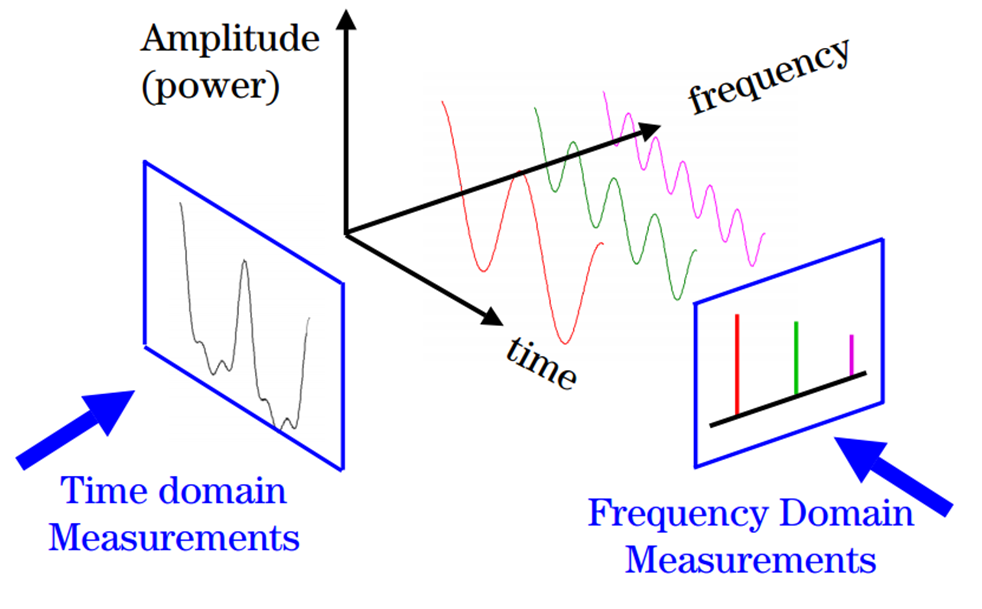
\includegraphics[width=4in]{amp-time-frequency}
	\caption{Conceptual comparison between time domain measurements (oscilloscope) and frequency domain measurements (spectrum analyzer)~\cite{thomas-sa}}
	\label{fig:amp-time-frequency}
\end{figure}

Fig.~\ref{fig:sa-screen} shows a screen capture of a typical spectrum analyzer measurement. The horizontal axis is frequency, and the vertical axis is signal power in dB scale. This figure shows a fairly narrow band signal at 1.8271\,GHz. The power of the signal is 2.06\,dBm.

\begin{figure}[h]
	\centering
	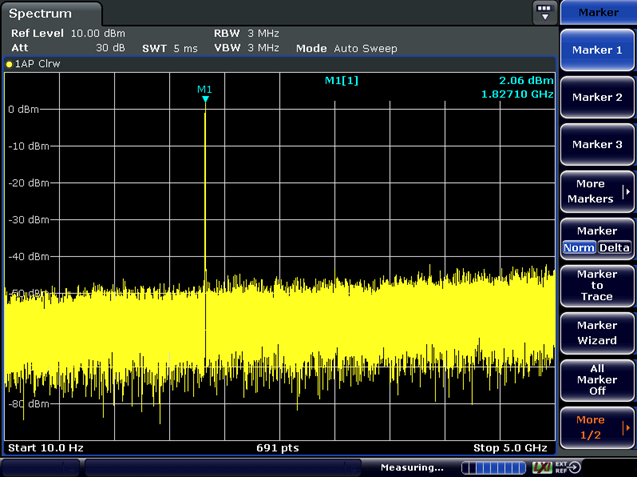
\includegraphics[width=4in]{sa-screen}
	\caption{Simplified block diagram of a spectrum analyzer.}
	\label{fig:sa-screen}
\end{figure}

At other frequencies where there is no input signal, we can still observe some measurement. As you might have guessed, these signals represent the noise, both from the signal source and from the spectrum analyzer itself. Obviously, it is important to have as low of a noise level as possible in order to detect extremely weak input signals. In fact, an important metric of a spectrum analyzer's performance is its sensitivity, i.e. the weakest signal that it can measure. This is often specified as \textit{Displayed Average Noise Level} (DANL), usually measured in dBm at the smallest \textit{resolution bandwidth} (RBW, we will come to this soon), or directly in dBm/Hz. The sensitivity is then simply DANL+SNR, where SNR is the minimum required \textit{signal to noise ratio}. For a top of the line spectrum analyzer, you can expect a DANL of close to -170\,dBm/Hz.

Another related metric is the \textit{dynamic range}, which refers to the power difference between the strongest and the weakest signal a spectrum analyzer can measure. Dynamic range is usually specified in dB. The absolute maximum dynamic range that a spectrum analyzer can achieve is the difference between the maximum allowable input power and the DANL. 
Sensitivity and dynamic range speak for the design and build quality of a spectrum analyzer. However, the achievable sensitivity and dynamic range in an actual measurement are usually lower than the maximum. It depends on what you want to measure and how you set up the spectrum analyzer. To understand this, we need to learn a bit more about how a spectrum analyzer works. 

The basic working principle of a typical spectrum analyzer is conceptually quite simple\footnote{The actual implementation of an instrument grade spectrum analyzer can be extremely complex to meet the high performance specs}. It is basically a glorified high frequency signal receiver. Fig.~\ref{fig:sa-blocks} shows a very simplified system diagram of a typical spectrum analyzer, highlighting its major blocks. The input signal is downconverted to a much lower frequency (usually several MHz) before it is captured by a power detector. The downconverter is represented by a mixer with a sweeping local oscillator (LO). The LO signal is swept through a span of frequency that can be set by the user; this sets the frequency span of the measurement. The downconversion of the signal allows it to be optimally conditioned for the detection circuitry. 

\begin{figure}[h]
	\centering
	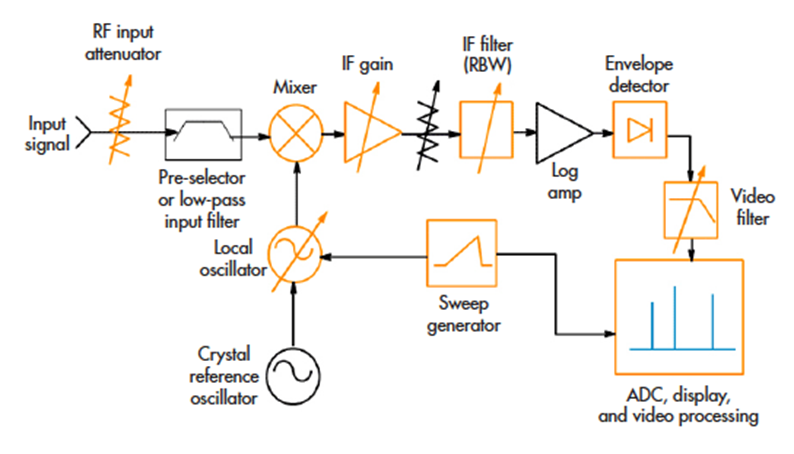
\includegraphics[width=4in]{sa-blocks}
	\caption{Simplified block diagram of a spectrum analyzer~\cite{diez-sa}.}
	\label{fig:sa-blocks}
\end{figure}

Before the downconverted signal enters the power detector, a narrow-band filter is used to allow only the desired signal to pass. This filter not only eliminates spurious signals but also limits the amount of noise power that enters the detector. As you can imagine, the narrower the filter passband is, the lower the noise floor would be. This filter is called the IF filter, and its bandwidth is called the resolution bandwidth (RBW). The power detector is effectively detecting the total power (signal plus noise) inside the resolution bandwidth. The best sensitivity and dynamic range of a spectrum analyzer can only be achieved with the narrowest RBW that is available in the instrument. Therefore, the available RBW bandwidth becomes an important metric itself. 

Besides affecting the noise floor, the RBW also has implications on how the signal looks on the screen. Consider the case of an ideal single-tone (meaning single frequency) input signal. The spectrum of this signal should look like a delta function in the frequency domain. Now imagine the receiver of the spectrum analyzer sweeps through the center frequency of the signal. Due to the finite width of the RBW, the measured spectrum will actually take the shape of the RBW filter! By carefully taking into the account of the RBW filter frequency response, the measured signal power and frequency can still be reconstructed. However, you would not be so lucky if you are dealing with more than one signals. Fig.~\ref{fig:sa-rbw} shows a scenario where three closely located signals cannot be reliably discerned by a large RBW. 

\begin{figure}[h]
	\centering
	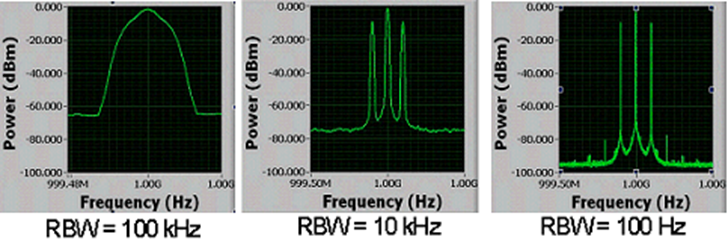
\includegraphics[width=4.5in]{sa-rbw}
	\caption{Small RBW resolves closely located signals.}
	\label{fig:sa-rbw}
\end{figure}

It becomes clear that an infinitely narrow IF filter is needed to faithfully reconstruct the true spectrum of the input signal. Obviously such a filter does not exist, and you will always have to keep in mind the broadening of the spectrum in a spectrum analyzer measurement. 

This simplistic introduction to spectrum analyzers will end here. There are obviously much more to learn about this fundamental high frequency signal characterization tool. To get a deeper understanding of spectrum analyzers and the principles of spectrum analysis, the following documents are recommended as further reading materials. 

\begin{itemize}[itemsep=0.1ex]
	\item ``Spectrum analysis basics,'' Agilent application note AN-150.
	\item ``Fundamentals of Real-Time Spectrum Analysis,'' Tektronix application note.
	\item Rigol DSA1030A-TG3 spectrum analyzer review and experiments (Video\footnote{This Youtube channel features many great tutorial videos related to high frequency electronics.}):\\  \url{https://www.youtube.com/watch?v=lu2Uaj3ZcoA }
\end{itemize}

\subsection{Voltage regulator}
In the late 1880s, a heated battle over the best mechanism to transport electricity over long distance broke out between proponents of direct current (primarily Thomas Edison) and alternating current (primarily George Westinghouse and several European companies). History eventually settled on ac current as the preferred method for long distance distribution because of its ability to be easily transformed into high voltages to reduce resistive loss along the wires. So today we all have ac outlets at home and in the lab. However, most if not all the circuits we have studied in our curriculum are powered from dc supplies. Have you ever wondered how dc voltages are generated from an ac supply? The following videos may be instructive. Make sure you watch them carefully. 

\begin{itemize}[itemsep=0.1ex]
	\item How to build an AC-DC power supply:\\ \url{https://www.youtube.com/watch?v=cyhzpFqXwdA} 
	\item Linear voltage regulator:\\ \url{https://www.youtube.com/watch?v=GSzVs7_aW-Y}
	\item Adjustable linear voltage regulator:\\  \url{https://www.youtube.com/watch?v=IjJWWGPjc-w}
	\item Switch-mode voltage regulator:\\ \url{https://www.youtube.com/watch?v=CEhBN5_fO5o}
\end{itemize}

\subsection{DAC and ADC}

DAC and ADC are the interface between the analog and the digital world. A DAC takes digital input (``1''s and ``0''s) and convert them into an analog signal. An ADC does the just the inverse of that, converting an analog signal into a digital one. A simple DAC can be built with only resistors, such as the R-2R ladder shown in Fig.~\ref{fig:dac-adc}-a. A simple ADC is not much more complex using a linear resistor ladder integrated with comparator and decoders (Fig.~\ref{fig:dac-adc}-b)\footnote{A variety of other architectures exist for both DACs and ADCs with respective advantages and disadvantages.}




To learn more about DACs and ADCs, watch the following video and read the following documents. 

\begin{itemize}[itemsep=0.1ex]
	
	\item humanHardDrive, ``Electronics 201 -- Analog/Digital Conversion,''\\ \url{https://www.youtube.com/watch?v=cjmcAE1L6OQ}
	\item Bill McCulley, ``\href{https://github.com/ucdart/UCD-EEC134/blob/c58efc438dba2679658333c34c4a6f733f594b39/labs/lab1/references/%5BMcCulley2010%5D.DAC.Introduction.pdf}{Bridging the divide: Part I - DAC Introduction}\footnote{Following the link  will lead you to EEC134's repository on Github. If you want the actual PDF file, you can clone the entire repository to your harddrive. The file is under the foler /labs/lab1/references/.},'' National Semicondcutor, 2010
	\item Chris Pearson, ``\href{https://github.com/ucdart/UCD-EEC134/blob/e977e88aaaf67f53cd562d2a071746a38ea19aa3/labs/lab1/references/%5BPearson2012%5D.High.Speed.Analog.to.Digital.Converters.Basics.pdf}{High Speed, Digital to Analog Converters Basics},'' Texas Instruments, 2012.
	\item Mike Kester, ``\href{http://www.analog.com/media/en/training-seminars/tutorials/MT-019.pdf}{DAC Interface Fundamentals},'' Analog Devices, 2008.
	\item Chris Pearson,  ``\href{https://github.com/ucdart/UCD-EEC134/blob/da59c17c776faf159aaea506ebd87510907dc133/labs/lab1/references/%5BPearson2011%5D.High-Speed.Analog-to-Digital.Converter.Basics.pdf}{High-Speed, Analog-to-Digital Converters Basics},'' Texas Instruments, 2011.
\end{itemize}

\subsection{Serial interface}

For micro-controllers that don't have built-in DACs and/or ADCs, an external DAC/ADC IC needs to be used when conversion between analog and digital is required. Even micr-controllers with on-chip DAC/ADC may run into situations where more than conversions channels are needed. When using an external device, a digital interface for transmitting and receiving data is needed between the micro-controller and the device. 

Digital interface generally comes in two flavors: \textit{parallel} and \textit{serial}. In a parallel interface, each physical pin corresponds to one digital bit. For example, an 8-bit word would need 8 physical pins for transmission/reception. In a serial interface, the digital bits are transmitted/received sequentially in time and theoretically only two pins are needed (one for signal and one for ground). Depending on whether a clock is needed to time the transmission/reception of digital bits, serial interface can be further categorized into \textit{synchronous} and \textit{asynchronous}. For synchronous transmission, an additional pin for the clock signal would be needed.

Obviously, at the same physical bit rate\footnote{how often the voltage changes from logic $1$ to $0$ (or the other way) on a pin.}, parallel interfaces is much faster than a serial one. But the serial interface requires far less pins and therefore a smaller chip footprint and lower PCB routing complexity, both of which translates to lower cost!. Therefore, for medium to high rate (kp/s to a few Gp/s) data transmission, serial links are more popular.

In this class, we use synchronous serial interface, in particular the Serial Peripheral Interface (SPI) protocol, as the interface between micro-controllers and external devices, such as DACs, ADCs, and some other electronically controllable RF components. 

To learn more about the SPI interface, read the following documents:
\begin{itemize}[itemsep=0.1ex]
	\item Mike Grusin, ``\href{https://learn.sparkfun.com/tutorials/serial-peripheral-interface-spi}{Serial Peripheral Interface (SPI)},'' Sparkfun. \url{https://learn.sparkfun.com/tutorials/serial-peripheral-interface-spi}
	\item F.~Leens, ``\href{http://www.byteparadigm.com/applications/introduction-to-i2c-and-spi-protocols/}{Introduction to I²C and SPI protocols},'' Byte Paradigm, 2009. \url{http://www.byteparadigm.com/applications/introduction-to-i2c-and-spi-protocols/}
\end{itemize}

\subsection{Printed Circuit Board Design}
A major goal of this lab is to help you get familiar with printed circuit board (PCB) design techniques. There are numerous PCB design software packages available on the market. In this quarter, you will start with a simple tool called KiCad. Once you are familiar with the basic concepts, it is easier to transition to a more sophisticated tool, such as the Cadence Allegro which is made available to us by a donation from Cadence. 

KiCad is an open-source electronic design software with very good PCB layout capabilities. KiCAD is becoming more popular in the hobbyist electronics community because it doesn't have any restrictions on the number of layers or boards sizes, nor does it lock you down to a particular PCB manufacturer.

To learn how to use KiCad and design PCBs in general, please go through the following materials.

\begin{itemize}[itemsep=0.1ex]

	\item Video tutorials from Contextual Electronics:	 \url{https://www.youtube.com/playlist?list=PLy2022BX6Esr6yxwDzhqYZyuuenJE2s5B} 
	
	\item 	Video tutorials form  Yoonseo Kang:	 \url{http://vimeo.com/user9565582} 

	\item A simple KiCad example: 
	
	\url{http://exploreembedded.com/wiki/A_simple_example_for_beginners:_LED_Breakout} 
		
\end{itemize}

\reversemarginpar
\marginnote{\textbf{Pre-lab Assignment}\\\textbf{ 1.1} \\Due: \due{Sep.~25th, 2015}}  Please answer the following questions:
\begin{enumerate}[itemsep=0.1ex, label=\alph*)]
	\item What are the advantages and disadvantages of using switch mode voltage regulator vs a linear voltage regulator?
	\item For the circuit of Fig.~\ref{fig:lm317_prelab}, with sing an input voltage of 9V and R1=\SI{510}{\ohm}, what's the value of R2 such that the output voltage is 5\,V? What is the efficiency of the regulator in this case? ``LM317'' refers to the Texas Instruments LM317 voltage regulator IC. You should be able to find its datasheet online. 
	
	\begin{figure}[h]
	\centering
		\begin{circuitikz}[scale=0.75]
				\centering	
				\draw (0,0) to [short,o-] (1,0)
				(1,-0.5) rectangle (3,0.5)
				(3,0) to (3.5,0) to [R, l=$R_1$] (3.5,-2) to (2,-2)
				(2,-0.5) to (2,-2) to [R, l=$R_2$] (2,-4) node [sground]{}
				(3.5,0) to [short, -o] (4,0)
				(-1,0)	node []{input}
				(5,0) node []{output}
				(2,0) node []{LM317}
				;
			\end{circuitikz}
		\caption{LM317 linear regulator circuit.}
		\label{fig:lm317_prelab}
	\end{figure}
	
	\item According to the datasheet you found above, what is the typical drop out voltage for the TI LM317? If an input voltage of 12\,V is used, what range of output voltage can be considered regulated? 
	\item What is the maximum efficiency of the TI LM2694 switch mode voltage regulator for an output voltage of 5\,V? Under what conditions is this efficiency achieved? 
	
	\item What do \textit{LSB} and \textit{MSB} mean in a DAC? For a 12-bit DAC with an output reference voltage $V_{ref}$ of 2\,V, how much voltage does an LSB correspond to? What about a 24-bit DAC instead?
	

\end{enumerate}

\reversemarginpar
\marginnote{\textbf{Pre-lab Assignment}\\\textbf{ 1.2} \\Due: \due{Oct.~2th, 2015}}  Please answer the following questions:
\begin{enumerate}[itemsep=0.1ex, label=\alph*)]
	
	\item What does \textit{SFDR} mean for a DAC? What is the typical SFDR of the Analog Devices (ADI) AD9788 DAC? 

	\item What is the \textit{image} signal for a DAC output? If a DAC is operating at a clock rate of 200\,Msps and the output fundamental signal is a 50\,MHz sine wave, what are the frequencies of the first three images above the fundamental? 
	
	\item What does \textit{SNR} mean for a DAC? What is the typical SNR for the Linear Technology (Linear) LTC2641 DAC?
	
	\item What does \textit{THD} mean for an ADC? What is the typical THD for the TI ADS5400 ADC ?
	
	\item What does \textit{SINAD} mean for an ADC? What is the typical SINAD for the Linear LTM9008-14 ADC? 
	
	\item What does \textit{ENOB} mean for an ADC? How is it calculated? What is the ENOB for the Maxim Integrated (Maxim) MAX11270 ADC?
	
\end{enumerate}

\reversemarginpar
\marginnote{\textbf{Pre-lab Assignment}\\\textbf{ 1.3} \\Due: \due{Oct.~9th, 2015}}  Please answer the following questions:
\begin{enumerate}[itemsep=0.1ex, label=\alph*)]
	
	\item What is the highest speed 8-bit ADC you can find? What is its power consumption? What would be the power consumption of an 8-bit ADC with half of this speed?

	\item What is the frequency domain representation of the following triangle wave signal?
	\[
		x(t)=\sum_{k=-\infty}^\infty \left\{ \left(\frac{2t}{T}-\frac{kT}{2}\right)\Pi\left[\frac{2(t-k)}{T}\right] + \left(1-\frac{2t}{T}\right)\Pi\left[\frac{2(t-k-\frac{1}{2})}{T}\right] \right\},
	\]
	where $\Pi(t)$ is the rectangular pulse function
	\[
		\Pi(t) = \begin{cases}
					1 & 0\leq t \leq 1; \\
					0 & \text{elsewhere}. \\
				\end{cases}
	\]
	
	If we pass the signal through an ideal low-pass filter that keeps only the first three harmonics (including the fundamental, the 2nd harmonic, and the 3rd harmonic), what would the filter output signal look like in the time domain?
	
	\item Design an analog low-pass filter that meets the following specifications: 
		\begin{enumerate}
			\item In-band gain: 10\,dB;
			\item 3-dB cut-off frequency: 20\,kHz;
			\item Attenuation at 100\,kHz: 30\,dB.
		\end{enumerate}
	You may find online filter design tools, such as the TI \href{http://www.ti.com/lsds/ti/analog/webench/webench-filters.page}{WEBENCH Filter Designer\footnote{A short introduction video is available at \url{https://www.youtube.com/watch?v=bdtLbtfTV8A}}} and the ADI \href{http://www.analog.com/designtools/en/filterwizard/}{Filter Wizard}, to be useful. Verify the performance of your filter by simulation. You may use a SPICE simulator, such as \href{http://www.linear.com/designtools/software/}{LTSpice}, or a high frequency circuit simulator such as Agilent/Keysight Analog Design Systems (ADS). Both software are available on lab computers. 
	
\end{enumerate}

\newpage
\section{Equipment \& \\Supplies}

\begin{itemize}[itemsep=0.5ex]
\item breadboard
\item jumper wires
\item Arduino UNO development board
\item Teensy 3.1 development board (optional)
\item MCP4921 digital-to-analog converter (DAC)
\item misc resistors
\item misc capacitors
\item 8x AA rechargeable batteries
\item battery pack
\end{itemize}


%  \begin{steps}
%    \item First
%    \item Second
%    \item Third
%  \end{steps}

\newpage
\section{Procedures}

\subsection{Power supply/voltage regulator}

We will use a USB battery pack to power up our system. Batteries provide the cleanest (i.e. very little noise) type of supply but with one major disadvantage, their voltage keeps dropping due to increased internal resistance under discharge. A voltage regulator is therefore often used to provide a relatively stable dc voltage supply.

In our design, a LM317 adjustable regulator IC will be used to provide the supply voltages for several parts in the system. LM317 is a linear voltage regulator, which can provide a very clean output voltage and is quite simple to use. A linear regulator can only provide regulated output voltage lower than the primary voltage source. Another disadvantage of a linear regulator is its low efficiency when the difference between the input and output voltages is large. Because the same amount of current flows through the regulator and the load, the power being dissipated is roughly.

\begin{equation}
	P_d=I_{load}*\left( V_{in}-V_{out}\right)
\end{equation}

When the load current is high, this power dissipation can be significant. It is therefore important to provide good heat sinking to the regulator IC. In fact, many regulator ICs, such as the LM317,  have large exposed metal pad with low thermal resistance to facilitate mounting a heat sink.  However, it is very important to note that the metal pad on some regulator ICs, such as the LM317, is connected electrically to the output of the IC. If the heat sink may potentially come in contact with any other part of the circuit (including the enclosure, which often is tied to ground), proper isolation is needed between the IC and the heat sink. 
%
%When choosing a linear voltage regulator, several important specifications should be considered:
%\begin{itemize}[itemsep=0.5ex]
%	\item \textbf{Output voltage range}: the amount of ;
%	\item Maximum output current;
%	\item Drop-out voltage: this is the smallest voltage difference between the input and the output voltage before the output is no longer regulated. Having a low drop-out voltage is often advantageous;
%	\item Load regulation: the change in output voltage for a given change in load current;
%	\item Line regulation: the change in output voltage for a given input voltage change. 
%\end{itemize}

\begin{enumerate}
\item Using Fig.~\ref{fig:lm317_lab} as a reference, build the regulator circuit on the breadboard. You should be able to find the LM317 pinout diagram from its datasheet, which you find from online. \emph{As a general suggestion, it is important to keep your circuit well laid out and keep the connecting wires as short as possible. Cut the wires to the right length if necessary.} Fig.xxx shows an example breadboard layout for the LM317 regulator circuit in this lab. 

	\begin{figure}[h]
	\centering
		\begin{circuitikz}[scale=1]
				\centering	
				\draw (-2,0) node [above]{$V_{in}$} to [short,o-] (1,0)
				(-1,0) to [C, l=$C_i${=}\SI{0.1}{\micro\farad}] (-1,-2) node [sground]{}
				(1,-0.5) rectangle (3,0.5)
				(1.4,0.1) node [scale=0.75]{V$_{\text{IN}}$}
				(2,0.75) node []{LM317}
				(2.55,0.1) node [scale=0.75]{V$_{\text{OUT}}$}
				(2,-0.3) node [scale=0.75]{ADJ}
				(3,0) to (3.5,0) to [R, l=$R_1${=}\SI{220}{\ohm}] (3.5,-2) to (2,-2)
				(2,-0.5) to (2,-2) to [vR, l=$R_2: \text{2K potentiometer}$] (2,-4) node [sground]{}
				(3.5,0) to [short, -o] (7,0) node [above]{$V_{out}$}
				(6,0) to [C, l=$C_o${=}\SI{1}{\micro\farad}] (6,-2) node [sground]{}
				;
			\end{circuitikz}
		\caption{Schematic of the voltage regulator circuit using LM317.}
		\label{fig:lm317_lab}
	\end{figure}

\item For testing the circuit, we will first use the lab bench power supply as our input power. Set the power supply voltage to 5\,V and connect it to the input of your voltage regulator circuit. Adjust the $R_2$ potentiometer until the output voltage is 4\,V. You can use the lab multimeter to measure the output voltage. 

\item Line regulation: 
	\begin{enumerate}
		\item Use the bench power supply as the input; set it at 7\,V;
		\item Adjust R2 until the output is 5\,V;
		\item Adjust the input voltage from 7\,V to 5\,V at 0.25\,V intervals, and then from 5\,V to 2\,V at 0.5\,V intervals, record the regulator output voltage using the multimeter; 
		\item Plot your results. In what input voltage range does the LM317 provide good line regulation? 
		\item What is the dropout voltage at various input voltages? Does it agree with the datasheet?
	\end{enumerate}
	
% load regulation:

\end{enumerate}

\subsection{Precision voltage reference}

In order to present a precise and stable reference for the DAC and the ADC, we will build a precision voltage reference circuit. In this circuit, we will use the TI LT1009 reference IC with 2.5\,V output voltage and less than $\pm$ 0.2\% initial accuracy (no calibration and adjustment). The LT1009 IC can be used as a two-terminal voltage reference although it does provide an optional 3rd terminal for $\pm 5$\% adjustment.

\begin{enumerate}
	\item Build the following circuit on your breadboard. 
	\item Verify that the output voltage of the circuit is 2.5\,V.
\end{enumerate}

\subsection{Function generator}

There are numerous ways to build a function generator. You can use a 555 timer, a ring of inverters, dedicated oscillator ICs, or a direct digital synthesis (DDS) circuit which uses high-speed digital circuits to implement fast waveform generators. It does so by outputting values from a look-up table (LUT), which stores the desired waveform in discretized values, and converting them to an analog signal by a DAC. 

In this lab, we will try to emulate a DDS using a micro-controller and an MCP4921 DAC. We are interested in generating a triangle wave which will be useful in later labs. Since DAC outputs are discrete in nature, we are really just approximating the triangle wave with a stair-case waveform (Fig.~\ref{fig:tri_dac}). Obviously, the higher the resolution of the DAC, the better this approximate is. 

For this class, we will use the \textit{Teensy 3.1} micro-controller. The Teensy 3.1 is developed by Paul J.~Stoffregen of \href{https://www.pjrc.com}{PJRC.com}. The programming of Teensy 3.1 is done in the same IDE as the Arduino platform\footnote{with an add-on called Teensyduino, which has already been installed on the lab computer} and most Arduino programs will run without any problem on the Teensy. Compared to most Arduinos, however, the Teensy 3.1 has a much faster micro-controller (72\,MHz, overclockable to 96\,MHz) with floating point support and is therefore a much better platform than Arduinos if some number crunching is needed. 

\begin{figure}[h]
	\begin{tikzpicture}
		\draw (0,0) to [->|] (10,0);
		\draw (0,0) to [->|] (0,4);
		\draw (0,0) to (3.3,3.3) to (6.6,0);
		\foreach \i in {0,...,10}
			\draw (\i*0.3,\i*0.3) to (\i*0.3+0.3,\i*0.3) to (\i*0.3+0.3, \i*0.3+0.3);
		\foreach \i in {11,...,21}
			\draw (\i*0.3,6.6-\i*0.3) to (\i*0.3+0.3,6.6-\i*0.3) to (\i*0.3+0.3, 6.3-\i*0.3);
	\end{tikzpicture}
	\caption{Approximating a triangle wave using the stair-case output of a DAC.}
	\label{fig:tri_dac}
\end{figure}

\begin{enumerate}
	\item Using Fig.~\ref{fig:uno_sch} as a reference, connect the Teensy to the MCP4921 DAC. Connect the MCP4921's VDD and VREF pins to the LM317 regulator's output (4\,V) and both AVSS and $\overline{\text{LDAC}}$ to ground. A \SI{0.1}{\micro\farad} and a \SI{1}{\micro\farad} capacitor could be used at VREF to minimize noise at the reference. Connect the Teensy with the computer using a USB cable, which is used to program the Teensy and power it up.  It is very important to keep your circuit (ICs, resistors, capacitors, wires, etc) organized. Use as short of a wire as possible between two connection points. Refer to Fig.~\ref{fig:uno_pic} for an example layout. 

	\begin{figure}[h]
	\centering
		\begin{circuitikz}
				\centering	
				\draw (2, 0) rectangle (5,5)
				;
			\end{circuitikz}
		\caption{Schematic of the connection between Arduino UNO and the MCP4921.}
		\label{fig:uno_sch}
	\end{figure}

	\begin{figure}[h]
	\centering
		\begin{circuitikz}
				\centering	
				\draw (-2,0) node [above]{$V_{in}$} to [short,o-] (1,0)
				(-1,0) to [C, l=$C_i${=}\SI{0.1}{\micro\farad}] (-1,-2) node [sground]{}
				(1,-0.5) rectangle (3,0.5)
				(2,0) node []{LM317}
				(3,0) to (3.5,0) to [R, l=$R_1${=}\SI{220}{\ohm}] (3.5,-2) to (2,-2)
				(2,-0.5) to (2,-2) to [vR, l=$R_2$] (2,-4) node [sground]{}
				(3.5,0) to [short, -o] (7,0) node [above]{$V_{out}$}
				(6,0) to [C, l=$C_o${=}\SI{1}{\micro\farad}] (6,-2) node [sground]{}
				;
			\end{circuitikz}
		\caption{Connection of the Arduino and the DAC chip. Only the top DAC section of the breadboard needs to be assembled for this lab. Power supply is also not shown in this figure.}
		\label{fig:uno_pic}
	\end{figure}

\item Once the circuit is built, open the Arduino IDE, create a new sketch, and input the code ``triangle.ino'' (\url{https://github.com/ucdart/UCD-EEC134/blob/master/Lab1/triangle.ino}). \textbf{Make sure you read through and understand the code.} You may want to read the datesheet of MCP4921 to understand its SPI control protocol. 

\item Compile and upload the code to the Teensy. Use the following settings under the ``Tools'' menu: 
	\begin{enumerate}
		\item Board: ``Teensy 3.1''
		\item USB Type: ``Serial''
		\item CPU Speed: ``96\,MHz Optimized (Overclocked)''
	\end{enumerate}

\item In your report, include a screen capture of both the triangle (at VOUTA) and sync (at SYNC) output signals on the oscilloscope. Record their amplitudes and periods.

\item Disconnect the VREF pin of the DAC from the 5\,V regulator and connect it to an external 2.5\,V supply. How does changing the reference voltage affect the output signal?

\item How can you modify the code to change the amplitude and period of the output waveform? What is the fastest triangle wave you could generate? What do you think is the limitation to going even faster?

\item Modify the code to generate a sinusoidal wave. What is the highest frequency sinusoidal wave you can generate? The following link may give you some hint. 
\url{http://interface.khm.de/index.php/lab/experiments/arduino-dds-sinewave-generator/} 

%\item \textbf{(Challenge!)} Research and propose a design that will allow you to generate a 100\,kHz triangle and/or sine wave. (Hint: look-up table)

\item The Teensy actually has a built-in DAC. Try to implement the triangle wave generator using the built-in DAC. Refer to \url{https://www.pjrc.com/teensy/teensy31.html} for some hint. 

\item Write a sketch to generate a 10\,kHz triangle wave with at least 8-bit amplitude resolution. 
\end{enumerate}

\subsection{Low-pass filter}

In this part of the lab, we will implement an active low pass filter (LPF) with an adjustable gain stage. In the final radar system, the LPF+Gain stage will be responsible for filtering out spurious signals that may disturb the received baseband radar signals. Fig.~\ref{fig:lpf_sch} shows the schematic of the circuit. Fig.~\ref{fig:lpf_pic} shows an example of the actual circuit on a breadboard. 

The filter has a cut-off frequency of 15\,kHz. 

%It also filters out any spurious signals above a certain threshold frequency (15\,kHz in this design). To get the maximum resolution from the digitizer, the maximum strength of the signal should be less than the allowed input voltage range of the digitizer. 

%In our simple radar system, we are going to use the soundcard of the PC as the digitizer. The amplified and filtered IF signal is fed to the right channel of an audio card, which is conventionally connected using the red wire of a 3.5\,mm stereo jack or the ring of the connector (Fig. 6.10.3). 



\subsubsection{Gain stage}

We will use the Texas Instrument OPA4228 quad Op-Amp for both the gain stage and the active LPF. A pinout diagram of OPA4228 is shown in Fig. 6.10.4.

Identify the gain stage of the audio amplifier from Fig. 6.10.1. What is the expression of its gain? Notice the +5V bias does not affect this result, rather it simply shifts the bias of the overall amplifier since a single 9V supply (battery) is used vs a double +/- supply.
Build just the gain stage of the audio amplifier. Remember to power the op-amp chip by using 9V for V+ and ground for V-. Use the 9V battery as the supply for all the measurements to achieve better noise performance. Remember to disconnect the battery when measurements are not being made.
The gain is controlled using a 20\,k\si{\ohm} potentiometer (POT). To test the circuit, input a 1-kHz 10\,mVpp sine wave to the IF input using a signal generator. What is the maximum gain before clipping occurs, and what is the corresponding peak-to-peak voltage at the output?
The audio card on a typical laptop is designed to take in line level signals. Notice that this limits the sound card input signal strength to approximately 3 Vpp. Adjust the pot to achieve 3 Vpp on the oscilloscope at 1 kHz. Tabulate and plot the gain from 100\,Hz to 1\,MHz while keeping the pot fixed. Find the 3-dB cutoff frequency or the 3\,dB bandwidth at this gain. Use at least 20 data points.

\subsubsection{Active LPF}
Build the rest of the audio amplifier circuit, i.e. the active LPF. To measure just the filter response, disconnect R4 and R14 from the circuit (Fig. 6.10.1). Input a 3\,Vpp signal in place of R4 and measure the output in place of R14. R14 will only be needed as a current limiting resistor when connecting the amplifier to the laptop’s audio card. Again tabulate and plot the frequency response from 100 Hz to 20 kHz. What is the cutoff frequency of the filter?
The overall filter consists of 2 low pass filters. What is the order of the overall filter and how is it determined from the schematic? Is the bandwidth of the filter tunable? How would one increase or decrease the cutoff frequency?
What limitation does the cut-off frequency of the LPF place on the radar’s performance?  (Hint: what happens when your object is too far away)

\subsubsection{Gain Stage + Filter}
Reconnect R4 (R14 is still disconnected) and measure the overall response of the amplifier. Input a 100 mVp-p sine wave to the IF input. Adjust the pot for a 3 Vp-p output at 1 kHz and once again sweep the frequency from 100 Hz to 20 kHz while tabulating the voltage output and the gain. What is the cutoff frequency? Compare the results to previous measurements. Tabulate and plot all of the results for the report.
Reconnect R14. Break the audio cable and connect the LPF output to the right channel and the SYNC signal (from the modulator) to the left channel. 


\subsection{Analog-to-digital converter}

\subsection{Signal processing}

Use teensy 3.1 to sample and process data? sounds like too much work...

Using the laptop

\subsection{PCB Design}

\begin{thebibliography}{9}

 
\bibitem{thomas-sa}
Jeff Thomas, Tom Holmes, Terri Hightower, ``Learn RF Spectrum Analysis Basics,'' Agilent Technologies, \url{https://www.jlab.org/uspas11/Reading/RF/RF%20Spectrum%20Analysis.pdf}.

\bibitem{diez-sa}
Erik Diez, ``The Fundamentals of Spectrum Analysis,'' Agilent Technologies, \url{http://electronicdesign.com/test-amp-measurement/fundamentals-spectrum-analysis}.


\end{thebibliography}

\end{document}